\graphicspath{{./chapters/chapter03/}}
\chapter{Байесовское и минимаксное оценивания параметров}

В предыдущей главе мы заметили, что крайне маловероятно получить равномерно лучшую оценку. Альтернативный вариант для сравнения функций риска - это интегрирование или вычисление максимума.

\begin{defn}
	Пусть $(\mathcal{X}, \mathcal{B}, \mathcal{P})$ - статистический эксперимент, $\mathcal{P}=\{P_{\vartheta} \mid \vartheta \in \Theta\}$ и $(\Theta, \mathcal{A}_{\Theta})$ -- измеримое пространство. Вероятностная мера $\pi$ на $\mathcal{A}_{\Theta}$ называется \textbf{\textit{априорным распределением}} для $\vartheta$. Для оценки $g \in \mathcal{K}$ и её риска $R(\cdot, g)$ функция
	
	\[ R(\pi, g)=\int_{\Theta} R(\vartheta, g) \pi(d\vartheta) \]
	называется \textbf{\textit{Байесовским риском}} $g$ относительно $\pi$. Оценка $g^* \in \mathcal{K}$ называется \textbf{\textit{Байесовской оценкой}}, если она минимизирует Байесовский риск по всем возможным оценочным функциям:
	\[R(\pi, g^*)=\inf_{g \in \mathcal{K}}R(\pi, g).\]
\end{defn}

\begin{rmrk} \
	\begin{enumerate}
		\item В байесовской интерпретации параметр $\vartheta$ является случайным, а точнее - реализацией случайной величины $\theta:(\Omega, \mathcal{A}) \rightarrow (\Theta,\mathcal{A}_{\Theta})$ с распределением $\pi$.
		\begin{align*}
		& (\Omega, \mathcal{A}, \mathbb{P}) \xrightarrow{X} (\mathcal{X}, \mathcal{B}) \\
		& \quad \theta \downarrow \\
		& (\Theta,\mathcal{A}_{\Theta})
		\end{align*}
		\item Функция $R(\pi, g)$ играет роль среднего значения по всем функциям риска, где возможные значения $\theta$ имеют вес соответственно их вероятностям. Распределение $\pi$ может быть интерпретировано как априорное знание статистика о неизвестном параметре.
	\end{enumerate}
\end{rmrk}

\begin{asmp}
	В дальнейшем пусть $(\Theta, \mathcal{A}_\Theta) = (\MR^l, \mathcal{B}^l)$ и $(\mathcal{X}, \mathcal{B})=(\MR^n, \mathcal{B}^n)$. Также мы обозначаем $Q^{X,\theta}$ в качестве распределения $(X, \theta)$ на $(\mathcal{X} \times \Theta, \mathcal{B} \otimes \mathcal{A}_\Theta)$ и $P_\vartheta$ в качестве условного распределения $X$ (при условии $\theta = \vartheta$):
	\[P_\vartheta =Q^{X|\theta=\vartheta}. \]
	Мера $\pi$ является маргинальным распределением $\theta$ под $Q^{X,\theta}$. Для совместного распределения $(X,\theta)$ правило итерированного ожидания (Следствие \ref{crlr1.15}) дает:
	\[Q^{X,\theta}(A) = \int_{\Theta} \int_{\mathcal{X}} 1_A(x, \vartheta) P_\vartheta(dx) \pi(d \vartheta)   .\]
	Следует также заметить, что существует \textbf{\textit{апостериорное распределение}} $Q^{\theta|X=x}$ случайной величины $\theta$ при условии $X=x$.
\end{asmp}

\begin{rmrk}
		В Байесовской статистике значения $\pi$ и $P_\vartheta$ интерпретируются следующим образом: перед экспериментом $\pi=Q^\theta$ -- предполагаемое статистиком распределение параметра $\vartheta$. После наблюдения $X(\omega) = x$ информация о $\theta$ изменяется с $\pi$ на $Q^{\theta | X=x}$. Для функции риска от $\gamma(\vartheta)$ используются следующие представления:
		\[
		\begin{aligned}
		R(\pi,g) & =\int_\Theta R(\vartheta, g) \pi(d\vartheta)=\int_{\Theta} \int_{\mathcal{X}} L(\gamma(\vartheta), g(x)) P_\vartheta(dx) \pi(d\vartheta)\\
		& = \int_{\Theta \times \mathcal{X}} L(\gamma(\vartheta), g(x)) Q^{X,\theta} (dx, d\vartheta) \\
		& = \int_{\mathcal{X}} \int_{\Theta} L(\gamma(\vartheta), g(x)) Q^{\theta | X = x} (d\vartheta) Q^X(dx) \\
		& = \int_{\mathcal{X}} R_{\pi}^x(g) Q^X(dx).
		\end{aligned}
		\]
		Величина
		\[R_{\pi}^x(g) :=\int_{\Theta} L(\gamma(\vartheta), g(x)) Q^{\theta | X = x} (d\vartheta)\]
		называется \textbf{\textit{апостериорным риском}} g при данном X=x.
\end{rmrk}

\begin{thm} \label{thm3.5} \
	\begin{enumerate}
		\item Оценка $g^*$ является Байесовской оценкой для $\vartheta$ тогда и только тогда, когда $g^*$ доставляет минимум апостериорному риску $R_{\pi}^{X}(g)$ $Q^X$-п.н.
		\[R_{\pi}^x(g^*)=\inf_{g \in \mathcal{K}}R_{\pi}^x(g)=\inf_{a \in \Theta} \int L(\vartheta, a) Q^{\theta \mid X = x}(d\vartheta). \]
		\item Пусть $\Theta \subset \MR$, $L(\vartheta, a) = (\vartheta - a)^2$ и $\int \vartheta^2 Q^{\theta \mid X = x}(d\vartheta) < \infty$ $Q^X$-п.н. Тогда Байесовская оценка для $\vartheta$:
		\[g^*(x)=\ME[\theta | X = x] = \int_{\Theta} \vartheta Q^{\theta \mid X = x}(d\vartheta)\]
	\end{enumerate}
\end{thm}
\begin{proof}
	\begin{enumerate}
		\item В соответствии с Замечанием 3.4, $R(\pi, g)$ достигает минимума по $g$ тогда и только тогда, когда $R_{\pi}^x(g)$ минимальна относительно $g$ $Q^X$-п.н. В частности, мы минимизируем по всем возможным оценкам. Если существует $g^*$, то эта оценка должна минимизировать $R_{\pi}^x(g)$ $Q^X$-п.н., в противном случае возможно построить оценку, доставляющую меньшее значение риска.
		\item В соответствии с Теоремой 1.25, величина $\int_\Theta(\vartheta - a)^2 Q^{\theta|X=x}(d\vartheta)$ минимальна, если $a=\ME[\theta|X=x]$.
	\end{enumerate}
\end{proof}


\begin{rmrk}
	Если $P_\vartheta \ll \mu$ с $\mu$-плотностью $f(x|\vartheta)$ и также $\pi \ll \nu$ с $\nu$-плотностью $h(\vartheta)$, то совместное распределение $(X,\theta)$ удовлетворяет:
	\[ Q^{X, \theta} \ll \mu \otimes \nu  \]
	с плотностью $f(x|\vartheta) h(\vartheta)$. Также, апостериорное распределение $Q^{\theta | X=x}$ обладает $\nu$-плотностью:
	\[ f(\vartheta | x) = \frac{f(x|\vartheta) h(\vartheta)}{\int_\Theta f(x|\vartheta) h(\vartheta) \nu (d\vartheta)}
	\]
	если знаменатель положительный. Апостериорный и Байесовский риски соответственно:
	\[ R_\pi^x(g) = \frac{\int_\Theta L(\vartheta, g(x))f(x|\vartheta) h(\vartheta) \nu (d\vartheta)}{\int_\Theta f(x|\vartheta) h(\vartheta) \nu (d\vartheta)} , \]
	\[ R(\pi, g)=\int_{\mathcal{X}}\int_\Theta L(\vartheta, g(x))f(x|\vartheta) h(\vartheta) \nu (d\vartheta) \mu(dx). \]	
\end{rmrk}

\begin{exmp} \
	
	Рассмотрим пример с оцениванием параметра биномиального распределения. Пусть $\Theta = (0, 1)$, $\mathcal{X}=\{0, \dots , n\}$:
	\[P_\vartheta(X=x)=\binom{n}{x}\vartheta^x (1-\vartheta)^{n-x}.\]
	Функция потерь: $L(x,y)=(x-y)^2$
	\begin{itemize}
		\item UMVU-оценка для $\vartheta$: $g(x)=\frac{x}{n}$ (экспоненциальное семейство)
		\[\Var_{\vartheta}(g(X))=\frac{\vartheta(1-\vartheta)}{n}.\]
		\item Пусть $\pi \sim \mathcal{U}(0,1)$.
		
				\begin{figure}[!htb]\centering
					\begin{minipage}{0.7\textwidth} Тогда
						\[f(x \mid \vartheta) = \binom{n}{x}\vartheta^x (1-\vartheta)^{n-x} 1_{\{0, \dots , n\}}(x)\]
						и априорная функция плотности распределения параметра:
						\[h(\vartheta)=1_{(0,1)}(\vartheta).\]
					\end{minipage}
					\begin{minipage}{0.18\textwidth}
						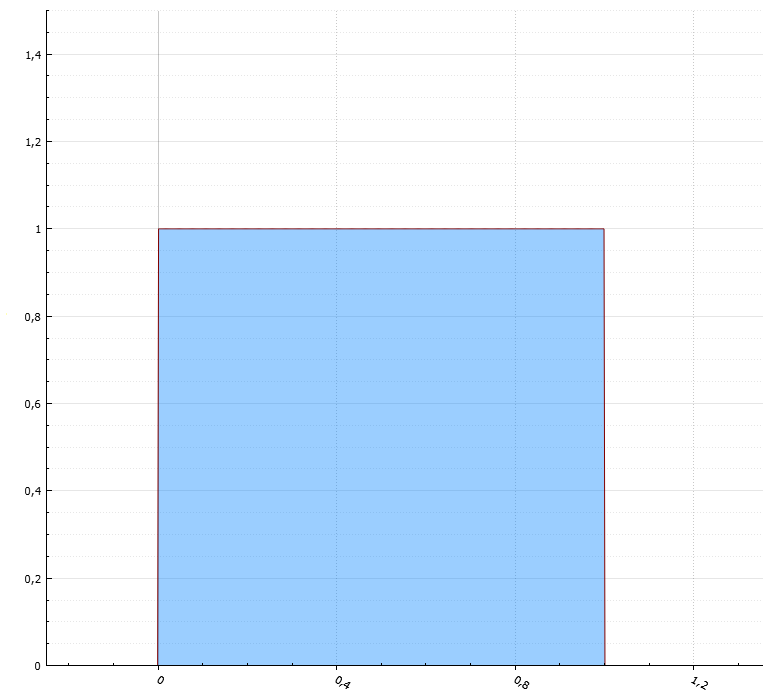
\includegraphics[width=\linewidth, right]{uniform}
						\captionsetup{labelformat=empty}
						\caption{$h(\vartheta)$}
					\end{minipage}
				\end{figure}
			
									
				\begin{figure}[!htb]\centering
					\begin{minipage}{0.7\textwidth}
						Апостериорная плотность вероятности:
						\[f(\vartheta \mid x) = \frac{\vartheta^x (1-\vartheta)^{n-x} 1_{(0,1)}(\vartheta)}{B(x+1, n-x+1)}, \]
						
						где в знаменателе бета-функция:
						\[B(a,b)=\int_{0}^{1} \vartheta^{a-1} (1-\vartheta)^{b-1} d \vartheta. \]
					\end{minipage}
					\begin{minipage}{0.18\textwidth}\centering
						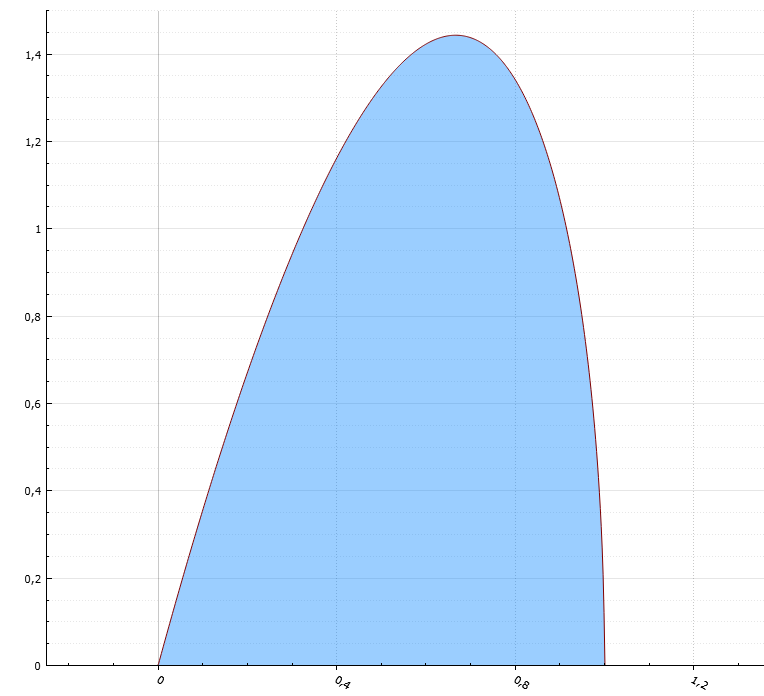
\includegraphics[width=\linewidth, height=2.6cm, right]{beta}
						\captionsetup{labelformat=empty}
						\caption{$f(\vartheta \mid x)$}
					\end{minipage}
				\end{figure}
			
			Тогда Байесовская оценка:
		\[g^*(x)=\ME[\theta|X=x]=\int_0^1 \frac{\vartheta^{x+1}(1-\vartheta^{n-x})}{B(x+1, n-x+1)}=\frac{B(x+2, n-x+1)}{B(x+1, n-x+1)} =\frac{x+1}{n+2},\]
		и Байесовский риск:
		\[
		\begin{aligned}
			R(\pi,g^*) & =\int_0^1 R(\vartheta, g^*) d\vartheta=\int_0^1 \ME_\vartheta\Big[\Big(\frac{X+1}{n+2}-\vartheta \Big)^2\Big]d\vartheta \\
			 & =\frac{1}{(n+2)^2} \int_0^1 (n\vartheta - n\vartheta^2+1-4\vartheta+4\vartheta^2)\ d\vartheta=\frac{1}{6(n+2)}.  
		\end{aligned}
		\]
	\end{itemize}
\end{exmp}

\begin{exmp}
	Пусть $X_1, \dots, X_n$ i.i.d. $\sim P_\mu^1=\mathcal{N}(\mu, \sigma^2)$ с заранее известным параметром $\sigma^2$. Априорное распределение $\mu$:
	\[ 
	h(\mu) = \frac{1}{\sqrt{2 \pi \tau^2}} \exp \Big\{ -\frac{(\mu-\mu_0)^2}{2\tau^2} \Big\}.
	\]
	Используя плотность распределения $X$
	\[
	f(x|\mu)=\Big( \frac{1}{\sqrt{2\pi \sigma^2}}\Big)^n \exp \Big\{ \frac{1}{2\sigma^2}\sum_{j=1}^n(x_j-\mu)^2 \Big \},
	\]
	получаем апостериорное распределение:
	\[  
	Q^{\mu|X=x} \sim \mathcal{N} \Big( g_{\mu_0, \tau^2}(x), \Big( \frac{n}{\sigma^2} + \frac{1}{\tau^2}\Big)^{-1}  \Big),
	\]
	где
	\[ 
	g_{\mu_0, \tau^2}(x)=\Big( 1 + \frac{\sigma^2}{n \tau^2} \Big)^{-1} \overline{x}_n+\Big( \frac{n \tau^2}{\sigma^2}+1 \Big)^{-1} \mu_0.
	\]
	Для квадратичного риска функция $g_{\mu_0, \tau^2}(x)$ -- Байесовская оценка. Интерпретация: при большом значении $\tau^2$ (мало априорной информации) оценка $g_{\mu_0, \tau^2}(x) \approx \overline{x}_n$, иначе $g_{\mu_0, \tau^2}(x) \approx \mu_0$.
\end{exmp}

\begin{defn}
	Пусть $g$ -- оценка $\gamma(\vartheta)$. Тогда:
	\[ R^*(g)=\sup_{\vartheta \in \Theta} R(\vartheta, g) \]
	называется \textbf{\textit{максимальным риском}} $g$ и
	\[ R^*(g^*)= \inf_{g \in \mathcal{K}} R^*(g) \]
	называется \textbf{\textit{минимаксным риском}}, а соответствующая оценка $g^*$ -- \textbf{\textit{минимаксной}}.
\end{defn}

\begin{rmrk} \
	\begin{enumerate}
		\item Использование минимаксной оценки нацелено на защиту от больших потерь.
		\item Пусть $\mathcal{M} = \{ \pi \mid \pi \text{ -- вероятностная мера на } \mathcal{A}_\Theta \}$. Тогда несложно заметить, что:
		\[ R^*(g)=\sup_{\pi \in \mathcal{M}} R(\pi, g). \]
	\end{enumerate}
\end{rmrk}

\begin{defn}
	Априорное распределение $\pi^*$ на $\mathcal{A}_\Theta$ называется \textbf{\textit{наименее благоприятным априорным}}, если
	\[ \inf_{g \in \mathcal{K}} R(\pi^*, g) \geq \inf_{g \in \mathcal{K}} R(\pi, g) \quad \forall \pi \in \mathcal{M}. \]
\end{defn}

\begin{thm} \
	\begin{enumerate}
		\item Если $g_\pi$ -- Байесовская оценка относительно $\pi$ и 
		\begin{equation} \label{eq3.2}
		 R(\pi, g_\pi) = \sup_{\vartheta \in \Theta} R(\vartheta, g_\pi),
		\end{equation}
		то $g_\pi$ -- минимаксная оценка.
		\item Если $g_\pi$ -- единственная Байесовская оценка относительно $\pi$, удовлетворяющая равенству \eqref{eq3.2}, то $g_\pi$ -- единственная минимаксная оценка.
		\item Если равенство \eqref{eq3.2} выполняется, то $\pi$ -- наименее благоприятное априорное распределение.
	\end{enumerate}
\end{thm}

\begin{proof} \
	\begin{enumerate}
		\item Для любой оценки $g \in \mathcal{K}$:
		\[ \sup_{\vartheta \in \Theta}R(\vartheta, g) \geq \int_{\Theta}R(\vartheta, g)\pi(d\vartheta) \geq \int_{\Theta}R(\vartheta, g_\pi)\pi(d\vartheta)=R(\pi, g_\pi)=\sup_{\vartheta \in \Theta}R(\vartheta, g_\pi). \]
		\item Если $g_\pi$ -- единственная Байесовская оценка для $\pi$, то
		\[ \int_{\Theta} R(\vartheta, g)\pi(d\vartheta) > \int_{\Theta} R(\vartheta, g_\pi)\pi(d\vartheta) \quad \forall g \neq g_\pi. \]
		Тогда $\sup_{\vartheta \in \Theta}R(\vartheta, g) > \sup_{\vartheta \in \Theta}R(\vartheta, g_\pi) $ и $g_\pi$ единственная минимаксная оценка.
		\item Для любого распределения $\mu \in \mathcal{M}$:
		\[ \inf_{g \in \mathcal{K}} \int_{\Theta} R(\vartheta, g)\mu(d\vartheta) \leq \int_{\Theta}R(\vartheta, g_\pi)\mu(d\vartheta) \leq \sup_{\vartheta \in \Theta} R(\vartheta, g_\pi) = R(\pi, g_\pi) = \inf_{g \in \mathcal{K}} \int_{\Theta}R(\vartheta, g) \pi(d\vartheta). \]
	\end{enumerate}
\end{proof}

\begin{rmrk}
	Иногда функция риска Байесовской оценки $g_\pi$ является постоянной:
	\[ R(\vartheta, g_\pi) = c \quad \forall \vartheta \in \Theta. \]
	Тогда
	\[ \sup_{\vartheta \in \Theta} R(\vartheta, g_\pi) = c = \int_{\Theta} R(\vartheta, g_\pi) \pi(d\vartheta) = R(\pi, g_\pi), \]
	равенство \eqref{eq3.2} выполняется, $g_\pi$ минимаксная оценка и $\pi$ -- наименее благоприятное априорное распределение.
\end{rmrk}

\begin{exmp} \label{exmp3.14}
	Пусть $\Theta = (0, 1)$, $\mathcal{X}=\{0, \dots, n \}$ и 
	\[ P_\vartheta(X = x) = \binom{n}{x} \vartheta^x (1-\vartheta)^{n-x}. \]
	Мы снова используем квадратичный риск и выбираем бета-распределение в качестве априорного:
	\[ h(\vartheta) = \frac{\vartheta^{a-1}(1-\vartheta)^{b-1}1_{[0,1]}(\vartheta)}{B(a, b)}. \]
	Апостериорное распределение $Q^{\vartheta|X=x} \sim B(x+a,n-x+b)$ с плотностью:
	\[ f(\vartheta | x)= \frac{\vartheta^{x+a-1}(1-\vartheta)^{n-x+b-1}1_{[0,1](\vartheta)}}{B(x+a,n-x+b)}.  \]
	Несложно доказать, что для случайной величины $Z$ с бета-распределением $B(p,q)$
	\[\ME[Z]=\frac{p}{p+q} \quad \text{и} \quad \Var(Z)=\frac{pq}{(p+q)^2(p+q+1)}.	\]
	Используя Теорему \ref{thm3.5}, получаем Байесовскую оценку для $\vartheta$:
	\[g_{a,b}(x)=\frac{x+a}{n+a+b}. \]
	Соответствующий ей риск:
	\[ R(\vartheta, g_{a,b})=\ME[(g_{a,b}(X)-\vartheta)^2]=\frac{\vartheta^2(-n+(a+b)^2+\vartheta(n-2a(a+b))+a^2}{(n+a+b)^2}. \]
	Если выбрать постоянные $a^*=b^*=\sqrt{n}/2$, то риск будет равен:
	\[ R(\vartheta, g_{a^*,b^*})=\frac{1}{4(\sqrt{n} + 1)^2}. \]
	Такой риск не зависит от $\vartheta$, а значит оценка
	$g_{a^*,b^*}(x) = \frac{x+\sqrt{n}/2}{n+\sqrt{n}}$
	является минимаксной и $B(a^*, b^*)$ -- наименее благоприятное распределение.	
\end{exmp}


\begin{defn}
	Пусть
	\[ r_\pi = \inf_{g \in \mathcal{K}}R(\pi, g), \quad \pi \in \mathcal{M}. \]
	Последовательность $(\pi_m)_{m \in \MN}$ в $\mathcal{M}$ называется \textbf{\textit{наименее благоприятной последовательностью априорных распределений}}, если
	\begin{enumerate}
		\item $\lim\limits_{m \rightarrow \infty} r_{\pi_m}=r,$
		\item $ \forall \pi \in \mathcal{M} \quad r_\pi \leq r.$
	\end{enumerate}
\end{defn}

\begin{thm} \label{thm3.16}
	Пусть $(\pi_m)$ в $\mathcal{M}$ последовательность, такая что  $r_{\pi_m} \rightarrow r \in \MR$. Также пусть существует такая оценка $g^* \in \mathcal{K}$, что:
	\[ \sup_{\vartheta \in \Theta} R(\vartheta, g^*) = r. \]
	Тогда:
	\begin{enumerate}
		\item $g^*$ -- минимаксная оценка,
		\item $(\pi_m)$ -- наименее благоприятная последовательность априорных распределений.
	\end{enumerate}
\end{thm}

\begin{proof} \
	\begin{enumerate}
		\item Для любой оценки $g \in \mathcal{K}$
		\[ \sup_{\vartheta \in \Theta} R(\vartheta, g) \geq \int_{\Theta}R(\vartheta, g)\pi_m(d\vartheta) \geq r_{\pi_m} \longrightarrow r=\sup_{\vartheta \in \Theta}R(\vartheta, g^*). \]
		\item Для любого распределения $\pi \in \mathcal{M}$
		\[ r_\pi \leq R(\pi, g^*)=\int_{\Theta} R(\vartheta, g^*) \pi(d \vartheta) \leq \sup_{\vartheta \in \Theta}R(\vartheta, g^*)=r. \]
	\end{enumerate}
\end{proof}

\begin{exmp}
	Пусть $X_1, \dots, X_n$ i.i.d. $\sim \mathcal{N}(\mu, \sigma^2)$ с известным параметром $\sigma^2$. В качестве априорного распределения выбираем:
	\[ h_m(\mu)=\frac{1}{\sqrt{2 \pi m}} \exp \Big \{ -\frac{(\mu-\mu_0)^2}{2m}\Big \}. \]
	Байесовская оценка:
	\[ g_m(x)=\Big( 1 + \frac{\sigma^2}{n m} \Big)^{-1} \overline{x}_n+\Big( \frac{n m}{\sigma^2}+1 \Big)^{-1} \mu_0.\]
	Для любого значения $\mu \in \MR$:
	\[  
	\begin{aligned}
	R(\mu, g_m) & = \ME_\mu[(g_m(X)-\mu)^2] \\
	& = \ME_\mu\Bigg[\bigg(\Big( 1 + \frac{\sigma^2}{n m} \Big)^{-1} (\overline{x}_n-\mu)+\Big( \frac{n m}{\sigma^2}+1 \Big)^{-1} (\mu_0-\mu)\bigg)^2\Bigg] \\
	& = \Big(1 + \frac{\sigma^2}{nm}\Big)^{-2} \frac{\sigma^2}{n} + \Big( 1+\frac{nm}{\sigma^2} \Big)^{-2}(\mu_0-\mu)^2 \xrightarrow[m \ \rightarrow \infty]{} \frac{\sigma^2}{n}
	\end{aligned}
	\]
	Так как риск ограничен сверху:
	\[ R(\mu, g_m) \leq \frac{\sigma^2}{n} + (\mu - \mu_0)^2, \]
	то по теореме Лебега о мажорируемой сходимости\footnote{
		Пусть фиксировано измеримое пространство $(X, \mathcal{F}, \mu)$. Предположим, что $\{ f_n \}_{n=1}^\infty$ и $f$ -- измеримые функции на $X$, причем $f_n(x) \rightarrow f(x)$ почти всюду. Тогда если существует определённая на том же пространстве интегрируемая функция $g$, такая что
		\[ |f_n(x)| \leq g(x) \quad \forall n \in \MN \]
		почти всюду, то $f_n$ и $f$ интегрируемы и
		\[ \lim\limits_{n \rightarrow \infty} \int_X f_n(x) \mu(dx) = \int_X f(x) \mu(dx). \]
		}:
	\[ r_{\pi_m}=R(\pi_m, g_m)=\int_{\MR}R(\mu, g_m)\pi_m(d\mu) \longrightarrow \frac{\sigma^2}{n}. \]
	Очевидно, $g^*(x)=\overline{x}_n$ удовлетворяет равенству
	\[ R(\mu, g^*)=\ME_\mu[(\overline{X}_n-\mu)^2]=\frac{\sigma^2}{n}, \]
	следовательно по Теореме \ref{thm3.16} $g^*$ -- минимаксная оценка и $\pi_m$ -- наименее благоприятная последовательность априорных распределений.
\end{exmp}

\raggedbottom
\pagebreak

\section*{Упражнения}
\begin{exc}
	Пусть $X \sim Po(\lambda)$ (распределение Пуассона). Функция потерь:
	\[ L(\lambda, a) = (\lambda - a)^2/\lambda. \]
	Докажите, что оценка $g(X)=X$ является минимаксной для параметра $\lambda$. Используйте следующие шаги:
	\begin{enumerate}
		\item Выберите гамма-распределение $\pi_{\alpha, \beta}=\Gamma(\alpha, \beta)$ в качестве априорного. Найдите апостериорное распределение.
		\item Рассчитайте апостериорный риск:
		\[ R_{\pi_{\alpha, \beta}}^x(a) := \int_{\Theta} L(\lambda, a) Q^{\lambda | X = x} (d\lambda). \]
		для $a \in \MR$ и $\alpha>1$. \\
		\subitem \textit{\textit{Подсказка}:} если $\Lambda \sim \Gamma(\alpha, \beta)$, то 
		\[ \ME[\Lambda]=\frac{\alpha}{\beta}, \quad \ME[1/\Lambda]=\frac{\beta}{\alpha-1}. \]
		\item Найдите значение $a^*$, доставляющее минимум апостериорному риску $R_{\pi_{\alpha, \beta}}^x(a)$. Рассчитайте соответствующий минимум $R_{\pi_{\alpha, \beta}}^x(a^*)$.
		\item Рассчитайте $R(\lambda, X)$ и тем самым завершите доказательство.
	\end{enumerate}
\end{exc}

\begin{exc}
	Докажите следующие утверждения:
	\begin{enumerate}
		\item Если $g^*$ -- допустимая оценка с постоянным риском, то $g^*$ -- минимаксная.
		\item Если $g^*$ -- Байесовская оценка для априорного распределения $\pi$ и единственная в том смысле, что для любой другой Байесовской оценки $\tilde{g}$
		\[ R(\vartheta, g^*)=R(\vartheta, \tilde{g}) \quad \forall \vartheta \in \Theta, \]
		то $g^*$ -- допустимая.
	\end{enumerate}
\end{exc}

\begin{exc}
	Пусть $X_1, \dots, X_n$ i.i.d. $\sim \mathcal{N}(\mu, \sigma^2)$, $X=(X_1, \dots, X_n)^T$ и функция потерь:
	\[ L(\sigma^2,d)=(d/\sigma^2-1)^2. \]
	Предположим, что $\mu=0$. Докажите, что
	\[ g(X)=\frac{1}{n+2}\sum_{i=1}^{n}X_i^2 \]
	является минимаксной оценкой $\sigma^2$. \\
	\subitem \textit{Подсказка}: произведите замену $\lambda=1/\sigma^2$ и возьмите для этого параметра априорное распределение $\pi_{\alpha, \beta}=\Gamma(p, b)$. Заметьте, что для апостериорного риска $g$:
	\[R_{\pi_{\alpha, \beta}}^x(\sigma^2, g)=\int_{\Theta}L(\sigma^2, g(x))Q^{\theta|X=x}d(1/\sigma^2)=\int_{\Theta}(g(x)\lambda-1)^2Q^{\theta|X=x}d(\lambda).\]
\end{exc}